\section{Introduction}


In Chapter \ref{ch:ReactionModels} we have established that our "Symmetric" and "Asymmetric" HDAC6 complex formation models are capable of predicting capsid breakage in normal and perturbed conditions. Here we attempt to apply them to make predictions about perturbed conditions which require further mechanistic investigation. One possible application has been suggested by the data provided by our collaborators from Patrick Matthias' group at FMI. They investigated designed ankyrin repeat proteins (DARPins) - artificial proteins which can bind target proteins with high affinity and specificity - and found that DARPin-F10 inhibits HDAC6-mediated influenza uncoating. We used their experimental insight about DARPin-F10 together with our established HDAC6 complex formation models to make predictions about DARPin-F10 effective concentrations and dose response in HDAC6 mediated influenza uncoating.

To compare our dose-response predictions with experimental DARPin-F10 viral growth data we sought out existing influenza infection models. To analyze the progression, severity, and duration of the infection, non-structured \textit{in vitro} influenza kinetic models use systems of ODEs describing cell populations interacting with the virus \cite{beauchemin2008modeling}. These models were considered a good fit for our goals, as they mostly rely on directly observed experimental quantities, such as viral growth. However, often the underlying fitting datasets are not collected with the goal of mathematical modelling in mind, which makes parameter identification a challenge \cite{boianelli2015modeling}.

Some of the newer studies describing structured and non-structured kinetic models \cite{rudiger2019multiscale, schulze2009infection} use attractive multi-dimensional datasets, which even without the use of the model may allow predictions of infection progression. Such datasets, when available, provide an intriguing opportunity to functionally characterise influenza infection, and make corresponding adjustments in our model structure. For example, it has long been established that high multiplicity of infection (MOI) tends to lead to higher synchrony of viral release \cite{cairns1957asynchrony}. For influenza kinetic models the parameters are often convoluted with other parameters or initial conditions. Thus, when the fitting dataset only includes a small variety of initial conditions, specifically with regard to initial virus concentration, it is difficult to judge how well the model would describe any other dataset.

In this chapter we give a brief summary of experimental data available for DARPin-F10 \cite{DarpinData} and provide an overview on \textit{in vitro} influenza kinetic modelling literature. We then model DARPin-F10 inhibition of HDAC6-Ub binding during influenza uncoating to predict active concentrations and dose-response behavior. We make use of available literature data \cite{rudiger2019multiscale, schulze2009infection} to analyze functional dependencies between model parameters, and to fit a simple influenza infection model, which we then use to model the effect of DARPin-F10 on influenza infection, and compare it to viral growth experiments.

\subsection{DARPin-F10 inhibits HDAC6-ZnF Ub binding}

\begin{figure}
\begin{center}
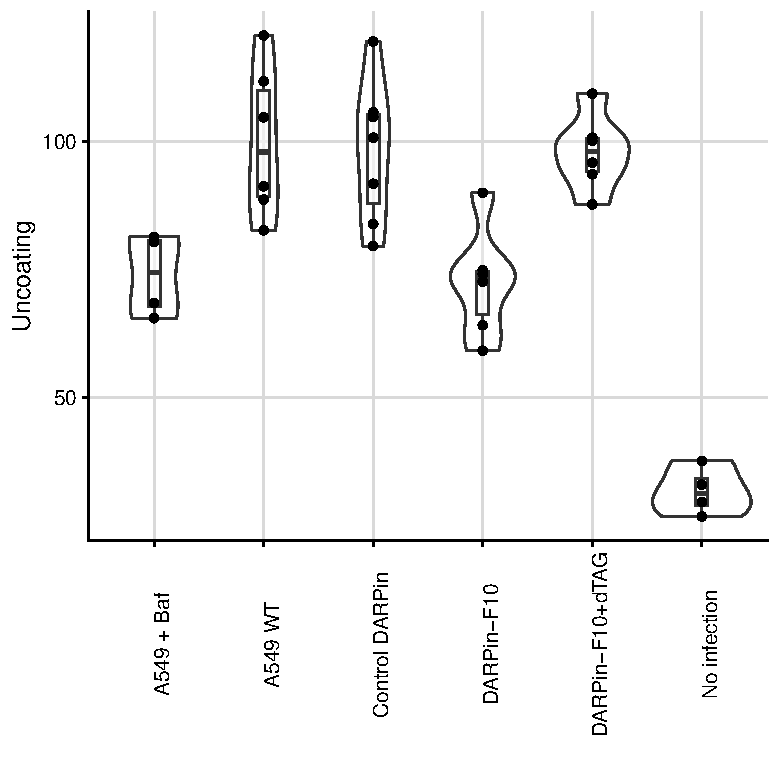
\includegraphics[width=0.95\textwidth, trim={0cm 0cm 0cm 0cm}, clip]{D_chapters/3_DARPinModels/DarpinUncoating.pdf}
\caption[DARPin-F10 reduces influenza virus uncoating]%
{DARPin-F10 reduces influenza virus uncoating at MOI = 30 PFU/ml.\par
A549 + Baf: the cells treated with Bafilomycin, an ATPase inhibitor which also stops viral uncoating;\par
A549 WT: wild type;\par
CTR DARPin: cells with a DARPin that did not bind anything;\par
DARPin-F10: cells with a DARPin that binds HDAC6 ZnF;\par
DARPin-F10 + dTAG: cells in which DARPin F10 was degraded through dTAG before virus infection;\par
* No infection: cells without any virus added to them.\par
All the values are normalized to A549 WT.}
\label{figure:darpinUncoatingExperimental}
\end{center}
\end{figure}

\begin{figure}
\begin{center}
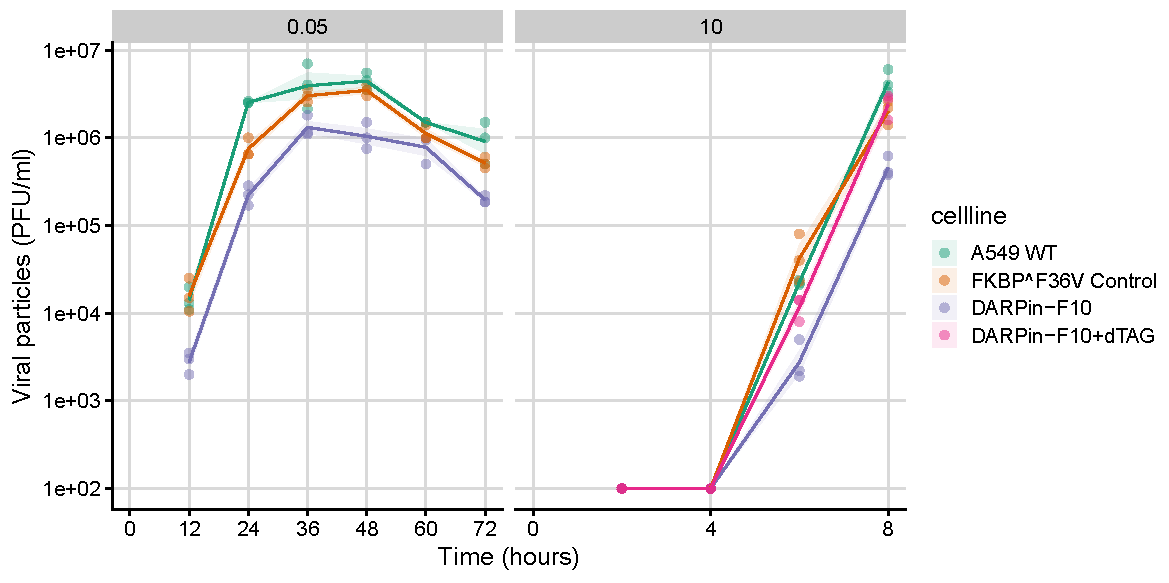
\includegraphics[width=0.95\textwidth, trim={0cm 0cm 0cm 0cm}, clip]{D_chapters/3_DARPinModels/DarpinVirusProduction.pdf}
\caption[DARPin-F10 reduces viral growth]%
{DARPin-F10 reduces viral growth at MOI = 0.05 and 10 PFU/ml.\par
A549 WT: wild type;\par
FKBP\textasciicircum F36V Control: cell line with a different mutation.\par
DARPin-F10: cells with a DARPin that binds HDAC6 ZnF;\par
DARPin-F10 + dTAG: cells in which DARPin F10 was degraded through dTAG before virus infection.}
\label{figure:darpinGrowthExperimental}
\end{center}
\end{figure}

Our collaborators from Patrick Matthias’ group at FMI showed that DARPin-F10 has a high specificity and affinity against HDAC6-ZnF \cite{DarpinData}. They were able to stably express and degrade DARPin-F10 in A549 cells in inducable manner. Using these new mutant cell lines they demonstrated that expression of DARPin-F10 for MOI = 30 plaque-forming units (PFU)/ml leads to the reduction in influenza viral uncoating (Figure \ref{figure:darpinUncoatingExperimental}), and for MOI 10 and 0.05 PFU/ml - to a reduction in virus production (Figure \ref{figure:darpinGrowthExperimental}) by about an order of magnitude.

Knowing that DARPin-F10 binds to HDAC6-ZnF we can reasonably assume that during influenza uncoating it acts as a competitor against polyubiquitin chains. In this chapter, we use that assumption, and introduce DARPin-F10 to our HDAC6 complex formation models.

\subsection{Influenza infection modelling}

Seasonal and zoonotic influenza is a popular subject of viral modelling, which has a variety of approaches. The majority of viral models use systems of ordinary differential equations (ODE), but partial (PDE) and delay differential equations (DDE) have also been implemented.

Influenza infection dynamic models are focused primarily capturing the transmission between hosts, with the goal of informing public health decisions and assist in pandemic planning \cite{ferguson2006strategies, mcvernon2007model}.

With the advancement of social media, a new type of influenza forecasting models has emerged \cite{pawelek2014modeling, santillana2015combining, levy2018modeling}, relying on publicly available self-reporting by users.

Structured models which include individual processes in virus replication \cite{sidorenko2004structured}, endosomal escape \cite{lagache2012modeling} and defective viral particle propagation \cite{rudiger2019multiscale} have been proposed. Their phenomenological nature means that they often rely on unobserved quantities and variables, and do not allow for inference on specific molecular targets for intervention.

Non-structured influenza kinetic models aim to understand and quantify the progression of the infection within a host or a cell culture, and resulting severity and duration \cite{beauchemin2008modeling}. This type of models has been used to help identify replication differences between different influenza strains \cite{simon2016avian}, impact of faulty viral particles on infection outcomes \cite{frensing2013continuous}, and effects of antiviral drugs on influenza infection \cite{beauchemin2008modeling, handel2007neuraminidase, holder2011assessing}. These models rely on directly observed experimental quantities for parameter fitting, however, often the datasets are reused, rather than collected with mathematical modelling in mind \cite{boianelli2015modeling}. \textit{In vitro} models usually have a simple and understandable structure, however, this simplicity makes inference and analysis of specific molecular targets largely impossible. \textit{In vivo} kinetic models build up on that basic structure and attempt to incorporate innate \cite{beauchemin2008modeling, handel2010towards,miao2010quantifying} and adaptive \cite{belz2002compromised, handel2010towards, miao2010quantifying} immune response. Here we primarily focus on \textit{in vitro} models, as our DARPin-F10 experimental data is coming from cell culture experiments.

The chronic infection kinetic model, originally proposed for human immunodeficiency virus (HIV) \cite{perelson2002modelling}, includes three states: $T$ - target cells, $I$ - infected cells, $V$ - viral particles, which are described as a system of ODEs:

\begin{equation}
\begin{array}{rcl}
\frac{dT}{dt} &=& s T - d T - \beta T V \\
\frac{dI}{dt} &=& \beta T V - \delta I \\
\frac{dV}{dt} &=& p I - c V
\end{array}
\end{equation}

where $s$ is target cells regeneration, $d$ is natural target cells death, $\beta$ is target cells infection rate by viral particles, $\delta$ is death rate of infected cells, $p$ is viral particle production rate by infected cells, and $c$ is clearance rate of viral particles.

It is often assumed that during acute ($s = d = 0$ \cite{baccam2006kinetics}) influenza infection target cells $T$ are limited and are depleted over the course of the infection:

\begin{equation}
\begin{array}{rcl}
\frac{dT}{dt} &=& - \beta T V \\
\frac{dI}{dt} &=& \beta T V - \delta I \\
\frac{dV}{dt} &=& p I - c V
\end{array}
\end{equation}

Another commonly made assumption is that during influenza infection viral production is delayed, which is accomplished through presence of latent eclipse phase infected cells $I_1$ and productively infected cells $I_2$ (\cite{baccam2006kinetics, smith2011effect}):

\begin{equation}
\begin{array}{rcl}
\frac{dT}{dt} &=& - \beta T V \\
\frac{dI_1}{dt} &=& \beta T V - k I_1 \\
\frac{dI_2}{dt} &=& k I_1 - \delta I_2 \\
\frac{dV}{dt} &=& p I_2 - c V
\end{array}
\end{equation}

where $k$ is a rate of $I_1$ maturation into $I_2$.

An alternative approach to modeling this latency is through the use of a system of delay differential equations (DDE), by introducing a fixed delay $\tau$:

\begin{equation}
\begin{array}{rcl}
&\frac{dT}{dt} = - \beta T(t) V(t) \\
&\frac{dI}{dt} = \beta T(t-\tau) V(t-\tau) - \delta I(t) \\
&\frac{dV}{dt} = p I(t) - c V(t)
\end{array}
\end{equation}

Here, during the "eclipse phase" the infected cell does not contribute to systems dynamics. A fixed delay model disregards variability of the transition time from eclipse phase, but allows to avoid unrealistically small or large transition times from the eclipse to productive phase \cite{beauchemin2008modeling}.

Models of viral production on microcarriers \cite{mohler2005mathematical,schulze2009infection} introduce a delay in the viral production term $p I(t - \tau)$ instead.

Several models have been suggested to describe influenza infection in presence of antiviral drugs. Amantadine drugs are commonly modelled as follows \cite{beauchemin2008modeling}:

\begin{equation}
\begin{array}{rcl}
\frac{dT}{dt} &=& - (1-\epsilon_{drug})\beta T V \\
\frac{dI}{dt} &=& \beta T V - \delta I \\
\frac{dV}{dt} &=& p I - c V
\end{array}
\end{equation}

where $\epsilon_{drug}$ is a drug efficacy, determined through a dose-response $E_{max}$ model:

\begin{equation}
\epsilon_{drug} = \epsilon_{max}\frac{1}{1 + (\frac{IC_{50}}{[D]})^{n}}
\end{equation}

where $\epsilon_{max}$ is a maximal drug effect such that $0 < \epsilon_{max} \le 1$, and $n \ge 0$ is a Hill coefficient.

In an alternative formulation, amantadine lengthens the eclipse phase instead of inhibiting the infection \cite{beauchemin2008modeling}:

\begin{equation}
\begin{array}{rcl}
\frac{dT}{dt} &=& - \beta T V \\
\frac{dI_1}{dt} &=& \beta T V - (1-\epsilon_{drug}) k I_1 \\
\frac{dI_2}{dt} &=& (1-\epsilon_{drug}) k I_1 - \delta I_2 \\
\frac{dV}{dt} &=& p I_2 - c V
\end{array}
\end{equation}

Similarly, neuraminidase inhibitors are often assumed to influence viral production rate $(1-\epsilon_{drug}) p I$ instead \cite{handel2007neuraminidase}.